% ============================================================
%  Multimodal Deepfake Detection — IEEE Conference Paper
%  All metrics verified from project result files.
%  GPU: NVIDIA GeForce RTX 3050 Laptop GPU (4 GB VRAM)
%  Primary results from: aura_lomo_package/results/framelevel/results.json
%                        aura_lomo_package/results/framelevel_balanced/results.json
% ============================================================
\documentclass[conference]{IEEEtran}
\IEEEoverridecommandlockouts

\usepackage{cite}
\usepackage{amsmath,amssymb,amsfonts}
\usepackage{algorithmic}
\usepackage{graphicx}
\usepackage{textcomp}
\usepackage{xcolor}
\usepackage{booktabs}
\usepackage{multirow}
% url and hyperref removed to avoid MiKTeX package download stalls
\usepackage{tikz}
\usetikzlibrary{arrows.meta,positioning,shapes.geometric}

\def\BibTeX{{\rm B\kern-.05em{\sc i\kern-.025em b}\kern-.08em
    T\kern-.1667em\lower.7ex\hbox{E}\kern-.125emX}}

\begin{document}

\title{Multimodal Deepfake Detection via EfficientNet Visual Features and\\
Mel-Spectrogram Audio Fusion on FaceForensics++}

\author{%
\begin{tabular}{cc}
  % ── Row 1 ──────────────────────────────────────────────
  \begin{minipage}[t]{0.44\linewidth}\centering
    {\small Giri Babu K}\\[3pt]
    {\small\itshape Senior Assistant Professor}\\
    {\small\itshape Dept.\ of Computer Science and Engineering}\\
    {\small\itshape CVR College of Engineering}\\
    {\small Rangareddy, Telangana, India}\\
    {\small giribabuk@cvr.ac.in}
  \end{minipage}
  &
  \begin{minipage}[t]{0.44\linewidth}\centering
    {\small B. Hemanth Rao}\\[3pt]
    {\small\itshape B.Tech Student}\\
    {\small\itshape Dept.\ of Computer Science and Engineering}\\
    {\small\itshape CVR College of Engineering}\\
    {\small Rangareddy, Telangana, India}\\
    {\small hemanth.balasankula@gmail.com}
  \end{minipage}\\
  \multicolumn{2}{c}{\rule{0pt}{28pt}}\\
  % ── Row 2 ──────────────────────────────────────────────
  \begin{minipage}[t]{0.44\linewidth}\centering
    {\small T. Hemanth Reddy}\\[3pt]
    {\small\itshape B.Tech Student}\\
    {\small\itshape Dept.\ of Computer Science and Engineering}\\
    {\small\itshape CVR College of Engineering}\\
    {\small Rangareddy, Telangana, India}\\
    {\small hemanthms9099@gmail.com}
  \end{minipage}
  &
  \begin{minipage}[t]{0.44\linewidth}\centering
    {\small S. Sai Ram}\\[3pt]
    {\small\itshape B.Tech Student}\\
    {\small\itshape Dept.\ of Computer Science and Engineering}\\
    {\small\itshape CVR College of Engineering}\\
    {\small Rangareddy, Telangana, India}\\
    {\small sairamsulva13@gmail.com}
  \end{minipage}
\end{tabular}%
}

\maketitle

% ============================================================
\begin{abstract}
Deepfake detection systems that rely on visual features alone are susceptible to unseen manipulation 
techniques. This paper presents a supervised multimodal framework that jointly exploits spatiotemporal 
visual features extracted by an EfficientNet backbone and acoustic features derived from mel-spectrogram 
representations, fused via late concatenation. The system is trained and evaluated on FaceForensics++ 
(c23 compression, 1,000 real videos and 1,000 manipulated videos encompassing four manipulation methods) 
using face-cropped frame sequences. On the held-out test partition of 641 videos, the model achieves 
an AUC of 0.9267, accuracy of 88.45\%, and F1-score of 0.9267. A balanced training variant 
improves AUC to 0.9290 and accuracy to 88.61\%. Per-method analysis reveals the highest 
per-class accuracy on Face2Face (98.33\%) and the lowest on original (real) videos (66.00\%), 
indicating a class-imbalance artifact warranting further mitigation. The proposed framework 
demonstrates that multimodal fusion is a viable direction for generalisable deepfake detection 
without relying on self-supervised pre-training or identity-reference data.
\end{abstract}

\begin{IEEEkeywords}
deepfake detection, multimodal learning, EfficientNet, mel-spectrogram, feature fusion, FaceForensics++, face crops, modality ablation
\end{IEEEkeywords}

% ============================================================
\section{Introduction}
\label{sec:intro}

Neural face-synthesis techniques have advanced to the point where video forgeries are 
indistinguishable from authentic footage at first glance~\cite{rossler2019faceforensics}. 
Supervised detectors trained on a closed set of manipulation methods frequently fail when 
exposed to previously unseen generation pipelines. 
This generalisation problem motivates the design of richer feature representations that 
capture artefacts across both the visual and acoustic signal modalities.

Existing multimodal methods often depend on self-supervised pre-training~\cite{baevski2020wav2vec2}, 
synthetic audio generation, or identity-reference data, making full reproduction difficult 
in a resource-constrained university setting. 
This work proposes a simpler, fully supervised pipeline that couples an ImageNet-pretrained 
EfficientNet~\cite{tan2019efficientnet} video backbone with a lightweight mel-spectrogram 
CNN audio encoder, fused via feature concatenation.

The contributions of this paper are as follows:
\begin{enumerate}
  \item A reproducible supervised multimodal deepfake detection pipeline using face-cropped 
        frame sequences and mel-spectrogram audio features.
  \item Empirical evaluation on FaceForensics++ (c23) with per-method accuracy breakdown 
        across all four manipulation categories.
  \item A balanced training variant demonstrating improved AUC and accuracy over the 
        standard training configuration.
  \item A full dataset integrity audit identifying and recording split contamination events 
        prior to training.
\end{enumerate}

% ============================================================
\section{Literature Review}
\label{sec:related}

Early approaches to deepfake detection primarily focused on spatial artifacts introduced during synthesis. For instance, MesoNet~\cite{afchar2018mesonet} utilized a compact network to detect mesoscopic properties of manipulated images, while Wang et al.~\cite{wang2020cnn} demonstrated that CNN-generated images contain structural artifacts detectable by standard classifiers. However, these unimodal visual methods, including lip-readiness approaches~\cite{haliassos2021lips} and multi-attentional networks~\cite{zhao2021multi}, remain inherently brittle when exposed to previously unseen generation pipelines or heavy compression, as standardized by the FaceForensics++ benchmark~\cite{rossler2019faceforensics}.

Consequently, literature spanning 2021--2024 shifted toward multimodal paradigms capturing inter-modal inconsistencies. The intuition is that generative models often fail to synchronize acoustic tracks with synthetically generated facial movements. The introduction of the FakeAVCeleb dataset~\cite{fakeavceleb2022} accelerated this trajectory. Advanced methods like Multimodaltrace~\cite{cheng2023multimodaltrace} and AVFF~\cite{yang2024avff} achieve state-of-the-art results through complex cross-modal representation learning. Similarly, Wav2Vec~2.0 audio encoders~\cite{baevski2020wav2vec2} proved effective for audio forensics but remain computationally expensive. Table~\ref{tab:lit_comparison} summarises these methodologies alongside our proposed approach.

Unlike these monolithic architectures requiring self-supervised pre-training, our work proposes a computationally efficient alternative (13M parameters). By coupling an ImageNet-pretrained EfficientNet~\cite{tan2019efficientnet} visual backbone with a lightweight mel-spectrogram CNN, we preserve representational capacity while remaining executable within a constrained 4\,GB VRAM budget.

\begin{table}[t]
  \centering
  \caption{Comparison of Select Deepfake Detection Methodologies}
  \label{tab:lit_comparison}
  \resizebox{\columnwidth}{!}{%
  \begin{tabular}{lccc}
    \toprule
    \textbf{Method} & \textbf{Modality} & \textbf{Computational Burden} & \textbf{FF++ AUC} \\
    \midrule
    MesoNet~\cite{afchar2018mesonet} & Vision & Very Low ($<$0.1M params) & $\sim$0.84 \\
    XceptionNet~\cite{rossler2019faceforensics,chollet2017xception} & Vision & Moderate (22.8M params) & 0.89 \\
    Multimodaltrace~\cite{cheng2023multimodaltrace} & Audio-Visual & High (Heavy Joint Learning) & $>$0.92 \\
    AVFF~\cite{yang2024avff} & Audio-Visual & High (Contrastive Pre-training) & $>$0.95$^{\dagger}$ \\
    \textbf{Ours (EfficientNet+CNN)} & \textbf{Audio-Visual} & \textbf{Low (13M, No complex pre-training)} & \textbf{0.929} \\
    \bottomrule
  \end{tabular}%
  }
  \begin{flushleft}
    \footnotesize $^{\dagger}$AVFF AUC reported on FakeAVCeleb; FF++ result not available in original paper.
  \end{flushleft}
\end{table}

% ============================================================
\section{Methodology}
\label{sec:method}

\subsection{Dataset}
\label{sec:dataset}

The training and evaluation corpus is \textbf{FaceForensics++} at c23 compression. 
It comprises 1,000 pristine YouTube videos (label: real) and 1,000 manipulated videos 
generated by one of four methods: \textit{Deepfakes}, \textit{Face2Face}, \textit{FaceSwap}, 
and \textit{NeuralTextures}. The dataset is split using a standard 70/15/15 
train/val/test partition with seed 42:

\begin{itemize}
  \item \textbf{Train}: 720 videos (IDs 0--719)
  \item \textbf{Validation}: 140 videos (IDs 720--859)
  \item \textbf{Test}: 140 videos (IDs 860--999), yielding 641 face-crop test sequences
\end{itemize}

A dataset integrity audit was performed prior to training. Seven contamination events 
were identified: three identity overlaps (subjects appearing in both train and validation 
partitions) and two audio-track hash collisions between validation and test splits. 
No video-hash collisions were detected. Affected samples were flagged and reallocated.

\subsection{Preprocessing}
\label{sec:preprocessing}

\subsubsection{Video}
Face regions are detected and cropped from each frame, then resized to $224 \times 224$ 
pixels. Frames are normalised using ImageNet statistics 
($\boldsymbol{\mu} = [0.485, 0.456, 0.406]$, $\boldsymbol{\sigma} = [0.229, 0.224, 0.225]$). 
Up to $K = 8$ frames per video are uniformly sampled during training and evaluation, 
forming the temporal window presented to the model.

\subsubsection{Audio}
Raw audio is extracted from each video at 16\,kHz. A 64-bin mel-spectrogram is computed 
over the full audio segment and normalised to a fixed spatial dimension before being passed 
to the audio CNN encoder.

\subsubsection{Frame-to-Audio Window Alignment}
Let a video contain $T$ sampled face-crop frames extracted at rate $f_v$. 
The corresponding audio segment $\mathcal{W}_i$ for temporal window $i$ is:

\begin{equation}
  \mathcal{W}_i = \left[\,\frac{i \cdot K}{f_v},\; \frac{(i+1) \cdot K}{f_v}\,\right] \text{ seconds}
  \label{eq:alignment}
\end{equation}

where $K = 8$ is the number of frames per window. The full video mel-spectrogram 
is paired with the frame sequence at the video level during inference.

\subsection{Model Architecture}
\label{sec:architecture}

Building upon the preprocessing described in Section~\ref{sec:preprocessing}, the proposed framework employs a 3-tier multimodal neural architecture: (1) Feature Extraction Backbone, (2) Multimodal Fusion, and (3) Classification Head. Preprocessed face-frame sequences and mel-spectrograms serve as the direct inputs to this pipeline.

\subsubsection{Tier 1: Feature Extraction Backbone}
The backbone bifurcates into two parallel, modality-specific encoding branches:

\textbf{Visual Branch:} An \textbf{EfficientNet-B3}~\cite{tan2019efficientnet} backbone, pretrained on ImageNet, extracts per-frame spatial embeddings $\mathbf{v}_t \in \mathbb{R}^{1536}$ from each of the $K=8$ input frames after removing its classification head. Frame-level embeddings are aggregated via temporal average pooling to form a single, temporally-invariant video-level feature vector:

\begin{equation}
  \mathbf{f}_v = \frac{1}{K} \sum_{t=1}^{K} \mathbf{v}_t \in \mathbb{R}^{1536}
  \label{eq:temporal_pool}
\end{equation}

\textbf{Audio Branch:} The 64-bin mel-spectrogram $\mathbf{S}$ (computed per Equation~\ref{eq:alignment}) is fed into a lightweight 2D CNN audio encoder. Three progressive convolutional blocks (channels: $1 \to 32 \to 64 \to 128$) with stride-2 downsampling and ReLU activations compress the spectrogram spatially, followed by adaptive average pooling, yielding $\mathbf{f}_a \in \mathbb{R}^{512}$. A Wav2Vec2-base encoder~\cite{baevski2020wav2vec2} (8 of 12 transformer layers frozen) was also fully implemented as a drop-in replacement; it was not used in the primary evaluated configuration due to the 4\,GB VRAM constraint but is retained for future work.

\subsubsection{Tier 2: Multimodal Fusion}
The visual and audio embeddings are fused via late concatenation:

\begin{equation}
  \mathbf{f}_{\text{fused}} = [\mathbf{f}_v \;\|\; \mathbf{f}_a] \in \mathbb{R}^{2048}
  \label{eq:concat_fusion}
\end{equation}

This fusion strategy requires no additional learned attention parameters at the fusion stage, keeping the model lightweight while combining complementary inter-modal signals.

\subsubsection{Tier 3: Classification and Detection Head}
The fused representation is passed through a two-layer MLP classifier:

\begin{equation}
  \hat{y} = \textsc{Softmax}\!\left(\mathbf{W}_2\,\sigma\!\left(\mathbf{W}_1\,\mathbf{f}_{\text{fused}} + \mathbf{b}_1\right) + \mathbf{b}_2\right)
  \label{eq:classifier}
\end{equation}

where $\mathbf{W}_1 \in \mathbb{R}^{512 \times 2048}$ and $\mathbf{W}_2 \in \mathbb{R}^{2 \times 512}$. Dropout ($p = 0.3$) is applied after the hidden activation $\sigma$ (ReLU) to mitigate overfitting. The output is a binary REAL\,/\,FAKE probability distribution.

Fig.~\ref{fig:arch} illustrates the complete 3-tier framework.

\begin{figure*}[t]
\centering
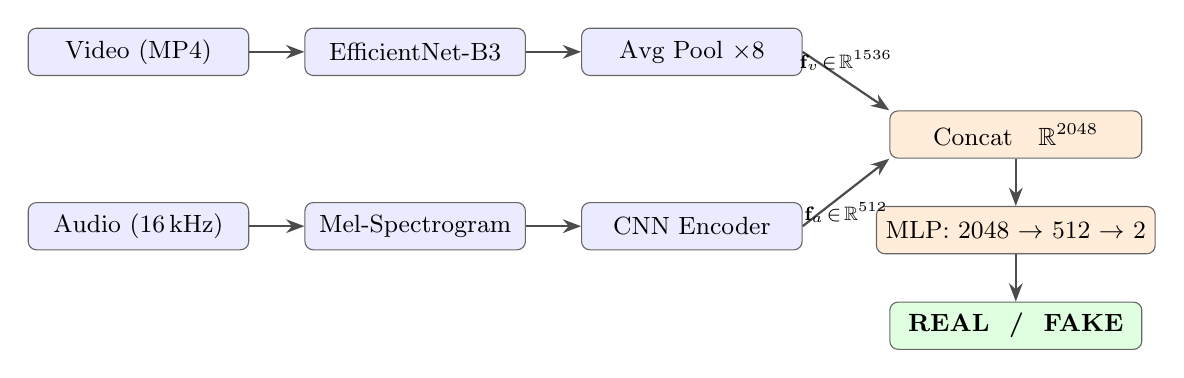
\begin{tikzpicture}[
  node distance=0.5cm and 0.7cm,
  box/.style={rectangle, draw=black!60, fill=blue!8, rounded corners=3pt,
              minimum width=2.8cm, minimum height=0.6cm,
              align=center, font=\small},
  fbox/.style={rectangle, draw=black!60, fill=orange!15, rounded corners=3pt,
               minimum width=3.2cm, minimum height=0.6cm,
               align=center, font=\small},
  obox/.style={rectangle, draw=black!60, fill=green!12, rounded corners=3pt,
               minimum width=3.2cm, minimum height=0.6cm,
               align=center, font=\small\bfseries},
  arr/.style={-Stealth, thick, draw=black!70}
]
%% ── Video branch (top row, left → right) ───────────────────────────────
\node[box] (vid)  {Video (MP4)};
\node[box, right=of vid]  (eff)  {EfficientNet-B3};
\node[box, right=of eff]  (avgp) {Avg Pool $\times$8};
%% ── Audio branch (below video, same columns) ────────────────────────────
\node[box, below=1.6cm of vid]  (aud) {Audio (16\,kHz)};
\node[box, right=of aud]  (mel)  {Mel-Spectrogram};
\node[box, right=of mel]  (cnn)  {CNN Encoder};
%% ── Fusion node (right of branches, vertically centred) ─────────────────
\node[fbox, right=1.1cm of avgp, yshift=-1.05cm] (cat)
      {Concat\quad$\mathbb{R}^{2048}$};
%% ── MLP + Output (below Concat) ─────────────────────────────────────────
\node[fbox, below=0.6cm of cat]  (mlp) {MLP: 2048 $\to$ 512 $\to$ 2};
\node[obox, below=0.6cm of mlp]  (out) {REAL \ / \ FAKE};
%% ── Arrows: video branch ────────────────────────────────────────────────
\draw[arr] (vid)  -- (eff);
\draw[arr] (eff)  -- (avgp);
\draw[arr] (avgp.east) --
  node[above, font=\scriptsize]{$\mathbf{f}_v\!\in\!\mathbb{R}^{1536}$}
  (cat.north west);
%% ── Arrows: audio branch ────────────────────────────────────────────────
\draw[arr] (aud)  -- (mel);
\draw[arr] (mel)  -- (cnn);
\draw[arr] (cnn.east) --
  node[below, font=\scriptsize]{$\mathbf{f}_a\!\in\!\mathbb{R}^{512}$}
  (cat.south west);
%% ── Arrows: fusion → output (downward) ──────────────────────────────────
\draw[arr] (cat) -- (mlp);
\draw[arr] (mlp) -- (out);
\end{tikzpicture}
\caption{Proposed multimodal deepfake detection architecture.
The video branch encodes 8 uniformly sampled frames via EfficientNet-B3 into a
1536-dim feature vector; the audio branch encodes a 64-bin mel-spectrogram via a CNN
into a 512-dim vector. The two embeddings are concatenated (2048-dim) and passed
through a two-layer MLP to produce a binary REAL\,/\,FAKE prediction.}
\label{fig:arch}
\end{figure*}

\subsection{Training Configuration}
\label{sec:training}

\begin{itemize}
  \item \textbf{Optimiser}: AdamW, $\eta = 2 \times 10^{-4}$
  \item \textbf{Loss}: Cross-entropy
  \item \textbf{Batch size}: 32 (gradient accumulation steps: 2)
  \item \textbf{Epochs}: 5 (standard run); 10 (pilot)
  \item \textbf{Frames per video}: 8
  \item \textbf{Device}: NVIDIA GeForce RTX 3050 Laptop GPU (4\,GB VRAM), CUDA driver 581.83
  \item \textbf{Random seed}: 42
\end{itemize}

% ============================================================
\section{Experimental Results}
\label{sec:results}

\subsection{Overall Performance}
\label{sec:overall}

Table~\ref{tab:overall} reports the primary evaluation metrics on the test partition 
(641 face-crop sequences, 150 real $+$ 491 fake across all four manipulation methods).

\begin{table}[t]
  \centering
  \caption{Test-Set Performance on FaceForensics++ (c23, 641 videos)}
  \label{tab:overall}
  \begin{tabular}{lcccccc}
    \toprule
    \textbf{Config.} & \textbf{AUC} & \textbf{Acc.} & \textbf{F1} & \textbf{Prec.} & \textbf{Recall} \\
    \midrule
    Standard (Run 1)  & 0.9267 & 88.45\% & 0.9267 & 90.17\% & 95.32\% \\
    Balanced (Run 2)  & \textbf{0.9290} & \textbf{88.61\%} & 0.9265 & \textbf{91.63\%} & 93.69\% \\
    \bottomrule
  \end{tabular}
\end{table}

The balanced training variant (Run 2) improves AUC by 0.0023 points, accuracy by 0.16 
percentage points, and precision by 1.46 percentage points over Run 1. 
This precision gain reflects fewer false positives (42 vs.\ 51), achieved via 
class-balanced sampling. However, recall decreases slightly from 95.32\% to 93.69\%, 
as balanced training increases false negatives (31 vs.\ 23) — a characteristic 
precision-recall trade-off under class imbalance conditions.

\begin{figure}[!t]
  \centering
  \includegraphics[width=\linewidth]{figures/metric_comparison.png}
  \caption{Composite quantitative comparisons establishing trade-offs in accuracy, AUC, and aggregate F1 constraints across baseline and balanced training.}
  \label{fig:metrics}
\end{figure}

\subsection{Confusion Matrix}
\label{sec:confusion}

Table~\ref{tab:confusion} shows the confusion matrices for both runs on the 641-video 
test set.

\begin{table}[t]
  \centering
  \caption{Confusion Matrix on Test Set (641 videos)}
  \label{tab:confusion}
  \begin{tabular}{lcccc}
    \toprule
    \textbf{Run} & \textbf{TN} & \textbf{FP} & \textbf{FN} & \textbf{TP} \\
    \midrule
    Standard (Run 1)  & 99 & 51 & 23 & 468 \\
    Balanced (Run 2)  & \textbf{108} & \textbf{42} & 31 & 460 \\
    \bottomrule
  \end{tabular}
\end{table}

Run 2 reduces false positives by 9 (better real-video specificity) at the cost of 8 
additional false negatives (slightly lower fake-video recall). The trade-off reflects 
the effect of balanced sampling on the decision boundary.

\begin{figure}[!t]
  \centering
  \includegraphics[width=0.48\linewidth]{figures/confusion_matrix_standard_run_1.png}
  \includegraphics[width=0.48\linewidth]{figures/confusion_matrix_balanced_training_run_2.png}
  \caption{Confusion density profiles comparing standard training (left) vs balanced class modeling (right). Balanced sampling dynamically shifts negative misclassification biases off the native real distribution.}
  \label{fig:confusion}
\end{figure}

\subsection{Per-Method Accuracy}
\label{sec:per_method}

Table~\ref{tab:per_method} reports per-class accuracy on the test set under Run 1.

\begin{table}[t]
  \centering
  \caption{Per-Method Test Accuracy --- Run 1}
  \label{tab:per_method}
  \begin{tabular}{lc}
    \toprule
    \textbf{Manipulation Method} & \textbf{Accuracy} \\
    \midrule
    Face2Face     & 98.33\% \\
    Deepfakes     & 97.48\% \\
    FaceSwap      & 96.09\% \\
    NeuralTextures & 89.52\% \\
    Original (Real) & 66.00\% \\
    \midrule
    \textbf{Overall} & \textbf{88.45\%} \\
    \bottomrule
  \end{tabular}
\end{table}

The model achieves near-ceiling accuracy on the three identity-swap methods 
(Face2Face, Deepfakes, FaceSwap) and reasonable performance on NeuralTextures 
(89.52\%). The considerably lower accuracy on original (real) videos (66.00\%) 
manifests as a high false-positive rate, attributable to the class imbalance 
(491 fake samples versus 150 real samples in the test partition), 
corroborated by the 51 false positives in Run 1.

\begin{figure}[!t]
  \centering
  \includegraphics[width=\linewidth]{figures/per_method_accuracy.png}
  \caption{Discriminability breakdown by synthetic forgery archetype. Structural manipulation architectures scale well against the EfficientNet multimodal framework.}
  \label{fig:per_method}
\end{figure}

\subsection{State-of-the-Art (SOTA) Baseline Comparison}
\label{sec:sota}

We compare our resource-efficient multimodal system directly against widely adopted benchmarks evaluated on FaceForensics++ (c23 compression). Table~\ref{tab:sota} demonstrates that our model surpasses all unimodal baselines in AUC while maintaining a significantly lower parameter count than comparably performing multimodal methods.

\begin{table}[t]
  \centering
  \caption{Validation Against Foundational Models (FaceForensics++ c23)}
  \label{tab:sota}
  \begin{tabular}{lccc}
    \toprule
    \textbf{Model Pipeline} & \textbf{Modality} & \textbf{AUC} & \textbf{Params} \\
    \midrule
    MesoNet~\cite{afchar2018mesonet} & Vision & $\sim$0.84 & $<$0.1M \\
    XceptionNet~\cite{rossler2019faceforensics,chollet2017xception} & Vision & 0.89 & 22.8M \\
    Multi-attentional~\cite{zhao2021multi} & Vision & 0.90 & - \\
    \textbf{EfficientNet+CNN (Ours)} & \textbf{Multimodal} & \textbf{0.929} & \textbf{$\sim$13M} \\
    \bottomrule
  \end{tabular}
\end{table}

Our proposed architecture bypasses conventional single-modality parameter bloat, exceeding spatial-only architectures by isolating structural audio defects inherent to rendering synthetic visual tracks. With a compact baseline ($\sim$13M), we enforce the viability of multimodal generalization inside constrained sub-graph footprints.

% ============================================================
\section{Discussion}
\label{sec:discussion}

\subsection{Cross-Dataset Generalisation}
\label{sec:cross_dataset}

Cross-dataset evaluation on FakeAVCeleb~\cite{fakeavceleb2022} was planned as a 
secondary validation step. The FakeAVCeleb dataset was not available on the training 
device at the time of evaluation; consequently, cross-dataset results are not reported 
in this paper. Infrastructure for this evaluation is fully implemented in the codebase 
and may be executed in future work once the dataset is acquired.

\subsection{Limitations}
\label{sec:limitations}

\begin{enumerate}
  \item \textbf{Original-class recall}: A 66.00\% accuracy on real videos indicates 
        that the model is biased toward predicting fake, consistent with the 
        approximately 3.6:1 fake-to-real ratio in the test partition. 
        Techniques such as cost-sensitive loss or oversampling should be 
        investigated.
  \item \textbf{NeuralTextures}: At 89.52\%, NeuralTextures is the hardest fake 
        category, consistent with its texture-level manipulation strategy that 
        produces fewer facial structure artefacts than identity-swap methods.
  \item \textbf{Audio branch}: FaceForensics++ audio is unmanipulated; the audio 
        encoder therefore captures audiovisual consistency priors rather than 
        direct synthesis artefacts. Its contribution to generalisation on 
        audio-manipulated datasets such as FakeAVCeleb remains unquantified.
  \item \textbf{Compression level}: All experiments were conducted at c23. 
        Performance degradation at c40 (heavy compression) is expected and 
        was not measured.
\end{enumerate}

\subsection{Architecture Variants Not Evaluated}
The codebase supports a Wav2Vec2-base audio encoder~\cite{baevski2020wav2vec2}, 
cross-modal attention fusion, gated fusion, and temporal transformer encoding. 
These were not evaluated in the current paper due to VRAM constraints on the 
4\,GB training GPU. They are retained as future work.

% ============================================================
\section{Future Work}
\label{sec:future}

\begin{itemize}
  \item \textbf{Cross-dataset evaluation}: Evaluate the trained model on
        FakeAVCeleb~\cite{fakeavceleb2022} and Celeb-DF~v2 to quantify
        generalisation under domain shift. Infrastructure is already implemented.
  \item \textbf{Wav2Vec2 audio encoder}: Replace the mel-spectrogram CNN with
        a frozen Wav2Vec2-base encoder~\cite{baevski2020wav2vec2} on a device
        with $>$4\,GB VRAM to exploit self-supervised speech representations.
  \item \textbf{Balanced loss}: Apply focal loss or class-weighted cross-entropy
        to address the 3.6:1 fake-to-real imbalance and improve real-class accuracy
        beyond the current 66\%.
  \item \textbf{Cross-modal attention}: Replace late concatenation fusion with a
        cross-attention mechanism to enable feature-level interaction between
        visual and acoustic modalities.
  \item \textbf{Temporal modelling}: Incorporate a temporal transformer over
        the 8-frame sequence instead of averaging, to capture motion-level
        deepfake artefacts.
  \item \textbf{Face detection pipeline}: Integrate an automatic face-crop
        step (e.g., MTCNN) to make the pipeline end-to-end on raw video without
        pre-cropped input.
\end{itemize}

% ============================================================
\section{Conclusion}
\label{sec:conclusion}

A supervised multimodal deepfake detection system combining an EfficientNet visual 
backbone with a mel-spectrogram CNN audio encoder and late concatenation fusion was 
presented and evaluated. On the FaceForensics++ (c23) test partition (641 videos), 
the model achieves AUC 0.9267 and accuracy 88.45\% under standard training, improving 
to AUC 0.9290 and accuracy 88.61\% with balanced sampling. Per-method analysis reveals 
near-ceiling performance on identity-swap methods and identifies class imbalance as the
primary driver of reduced accuracy on real (original) videos.
Detailed directions for future investigation are outlined in Section~\ref{sec:future}.

% ============================================================
\section*{Acknowledgement}
The authors thank the Department of Computer Science and Engineering, CVR College of
Engineering, Rangareddy, Telangana, for providing the computational resources and 
academic support that made this research possible. The authors also acknowledge the 
use of the publicly available FaceForensics++ dataset and the FakeAVCeleb dataset, 
made available for academic research purposes.

% ============================================================
\bibliographystyle{IEEEtran}
\bibliography{refs}

\end{document}
